%%%%%%%%%%%%%%%%%%%%%%%%%%%%%%%%%%%%%%%%%%%%%%%%%%%%%%%%%%%%%%%%%%%%%
% Mitschrieb vom 03.12.2013                                         %
%%%%%%%%%%%%%%%%%%%%%%%%%%%%%%%%%%%%%%%%%%%%%%%%%%%%%%%%%%%%%%%%%%%%%
\chapter{Fundamentalgruppe und Überlagerungen}
\section{Homotopie von Wegen}
\begin{figure}[ht]
    \centering
    \subfloat[$\gamma_1$ und $\gamma_2$ sind homotop, da man sie 
             \enquote{zueinander verschieben} kann.]{
        \documentclass[varwidth=true, border=2pt]{standalone}

\usepackage{pgfplots}
\usepackage{tikz}

\begin{document}
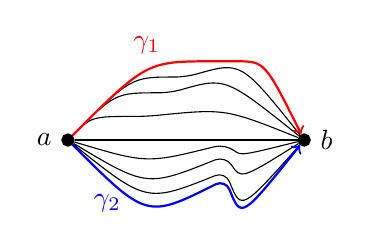
\begin{tikzpicture}
    \tikzstyle{point}=[circle,thick,draw=black,fill=black,inner sep=0pt,minimum width=4pt,minimum height=4pt]
    \node (a)[point,label=180:$a$] at (0,0) {};
    \node (b)[point,label=0:$b$]   at (3, 0) {};
    \draw [rounded corners] (a) .. controls (0.8,0.8) .. (1.5,0.8) .. controls (2.2,1) .. (b);
    \draw [rounded corners] (a) .. controls (0.6,0.6) .. (1.3,0.6) .. controls (2.0,0.8) .. (b);
    \draw [rounded corners] (a) .. controls (0.3,0.3) .. (1.0,0.3) .. controls (2.0,0.4) .. (b);
    \draw [rounded corners] (a) -- (b);
    \draw [rounded corners] (a) .. controls (1,-0.8) .. (2,-0.4) .. controls (2.2,-0.9) .. (b);
    \draw [rounded corners] (a) .. controls (1,-0.6) .. (2,-0.2) .. controls (2.2,-0.5) .. (b);
    \draw [rounded corners] (a) .. controls (1,-0.3) .. (2,-0.05) .. controls (2.2,-0.2) .. (b);
    \draw [rounded corners,->, thick, red] (a) .. controls (1,1) .. (2,1) .. controls (2.5,1) .. (b);
    \draw [rounded corners,->, thick, blue] (a) .. controls (1,-1) .. (2,-0.5) .. controls (2.2,-1) .. (b);
    \node at (1,1.2) [red] {$\gamma_1$};
    \node at (0.5,-0.8) [blue] {$\gamma_2$};
\end{tikzpicture}
\end{document}

        \label{fig:homotope-wege-anschaulich}
    }\hspace{1em}%
    \subfloat[$\gamma_1$ und $\gamma_2$ sind wegen dem Hindernis nicht homotop.]{
        \begin{tikzpicture}
    \tikzstyle{point}=[circle,thick,draw=black,fill=black,inner sep=0pt,minimum width=4pt,minimum height=4pt]
    \node (a)[point,label=180:$a$] at (0,0) {};
    \node (b)[point,label=0:$b$]   at (3, 0) {};
    \draw[orange,pattern color=orange,pattern=north east lines] (1.5,0) circle (0.3cm);
    \draw [rounded corners,->, thick, red] (a) .. controls (1,1) .. (2,1) .. controls (2.5,1) .. (b);
    \draw [rounded corners,->, thick, blue] (a) .. controls (1,-1) .. (2,-0.5) .. controls (2.2,-1) .. (b);
    \node at (1,1.2) [red] {$\gamma_1$};
    \node at (0.5,-0.8) [blue] {$\gamma_2$};
\end{tikzpicture}

        \label{fig:nicht-homotope-wege-anschaulich}
    }
    \label{Formen}
    \caption{Beispiele für Wege $\gamma_1$ und $\gamma_2$}
\end{figure}

\begin{definition}
    Sei $X$ ein topologischer Raum, $a, b \in X$, 
    $\gamma_1, \gamma_2: [0,1] \rightarrow X$ Wege von $a$ nach $b$,
    d.~h. $\gamma_1(0) = \gamma_2(0) = a$, $\gamma_1(1) = \gamma_2(1) = b$

    \begin{enumerate}[label=\alph*)]
        \item $\gamma_1$ und $\gamma_2$ heißen \textbf{homotop}\xindex{homotop},
              wenn es eine stetige Abbildung
              \[H(t,0) = \gamma_1(t), H(t,1) = \gamma_2(t) \;\;\; \forall t \in [0,1] =: I \]
              und $H(0,s) = a$ und $H(1,s) = b$ für alle $s \in I$ gibt.
              Dann schreibt man: $\gamma_1 \sim \gamma_2$

              $H$ heißt \textbf{Homotopie}\xindex{Homotopie} zwischen
              $\gamma_1$ und $\gamma_2$.
        \item $\gamma_s: I \rightarrow X, \gamma_s(t) = H(t,s)$ ist
              Weg in $X$ von $a$ nach $b$ für jedes $s \in I$.
    \end{enumerate}
\end{definition}

\begin{korollar}
    \enquote{Homotop} ist eine Äquivalenzrelation auf der Menge aller
    Wege in $X$ von $a$ nach $b$.
\end{korollar}

\begin{beweis}\leavevmode
    \begin{itemize}
        \item reflexiv: $H(t,s) = \gamma(t)$ für alle $t,s \in I \times I$
        \item symmetrisch: $H'(t,s) = H(t,1-s)$ für alle $t,s \in I \times I$
        \item transitiv: Seien $H'$ bzw. $H''$ Homotopien von $\gamma_1$
              nach $\gamma_2$ bzw. von $\gamma_2$ nach $\gamma_3$.

              Dann sei $H(t,s) := \begin{cases}
              H'(t, 2s)    &\text{falls } 0 \leq s \leq \frac{1}{2}\\
              H''(t, 2s-1) &\text{falls } \frac{1}{2} \leq s \leq 1\end{cases}$

              $\Rightarrow$ $H$ ist stetig und Homotopie von $\gamma_1$ nach 
              $\gamma_2$
    \end{itemize}
    $\qed$
\end{beweis}

\begin{beispiel}
    \begin{enumerate}[label=\arabic*)]
        \item Sei $X = S^1$. $\gamma_1$ und $\gamma_2$ aus 
              Abb.~\ref{fig:circle-two-paths} nicht homöotop.
              \begin{figure}
                \centering
                \documentclass[varwidth=true, border=2pt]{standalone}

\usepackage{pgfplots}
\usepackage{tikz}

\begin{document}
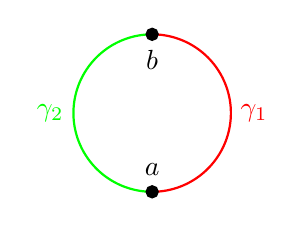
\begin{tikzpicture}
    \tikzstyle{point}=[circle,thick,draw=black,fill=black,inner sep=0pt,minimum width=4pt,minimum height=4pt]
    \draw [red,  thick,domain=90:-90,  samples=100] plot ({cos(\x)}, {sin(\x)});
    \draw [green,thick,domain=-90:-270,samples=100] plot ({cos(\x)}, {sin(\x)});
    \node (a)[point,label=90:$a$] at (0,-1cm) {};
    \node (b)[point,label=-90:$b$] at (0, 1cm) {};

    \node at (1,0) [anchor=180, red] {$\gamma_1$};
    \node at (-1,0) [anchor=0, green] {$\gamma_2$};

\end{tikzpicture}
\end{document}

                \caption{Kreis mit zwei Wegen}
                \label{fig:circle-two-paths}
              \end{figure}
        \item Sei $X = T^2$. $\gamma_1, \gamma_2$ und $\gamma_3$
              aus Abb.~\ref{fig:torus-three-paths} sind paarweise
              nicht homöotop.
              \begin{figure}
                \centering
                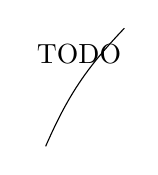
\begin{tikzpicture}
    \path (0,0)  edge [bend angle=10,bend right] node[label=TODO] {} (-1,-1.5);
\end{tikzpicture}

                \caption{Torus mit drei Wegen}
                \label{fig:torus-three-paths}
              \end{figure}
        \item Sei $X = \mdr^2$ und $a=b=(0,0)$. 

              Je zwei Wege im $\mdr^2$ mit Anfangs- und Enpunkt $(0,0)$
              sind homöotop.

              \begin{figure}
                \centering
                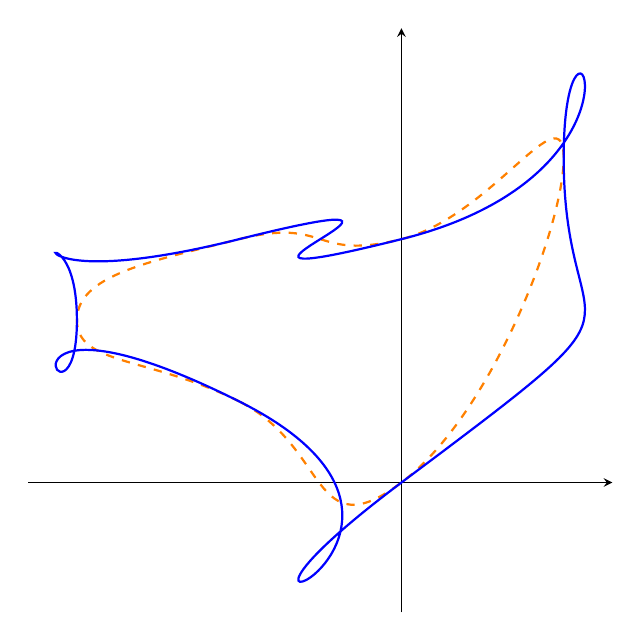
\begin{tikzpicture}
    \begin{axis}[
        legend pos=south west,
        axis x line=middle,
        axis y line=middle,
        %grid = major,
        width=9cm,
        height=9cm,
        grid style={dashed, gray!30},
        xmin=-2,     % start the diagram at this x-coordinate
        xmax= 1,    % end   the diagram at this x-coordinate
        ymin=-1,     % start the diagram at this y-coordinate
        ymax= 5,   % end   the diagram at this y-coordinate
        %axis background/.style={fill=white},
        %xlabel=$x$,
        %ylabel=$y$,
        ticks=none,
        %tick align=outside,
        %minor tick num=-3,
        enlargelimits=true,
        tension=0.08]
        \addplot[mark=none, orange, smooth cycle, thick, tension=1, dashed] coordinates {%
   (0,0) (-1,1) (-2,2) (-1,3) (0, 3) (1, 4)};
        \addplot[mark=none, blue, smooth cycle, thick, tension=3] coordinates {%
   (0,0) (-1,1) (-2,2) (-1,3) (0, 3) (1, 4)};
    \end{axis} 
\end{tikzpicture}

                \caption{Zwei Wege im $\mdr^2$ mit Anfangs- und Enpunkt $(0,0)$}
                \label{fig:torus-three-paths}
              \end{figure}

              Sei $\gamma_0: I \rightarrow \mdr^2$ der konstante Weg
              $\gamma_0(t) = 0 \; \forall t \in I$. Sei
              $\gamma(0) = \gamma(1) = 0$.

              $H(t,s) := (1-s) \gamma(t)$ ist stetig, 
              $H(t,0) = \gamma(t)\; \forall t \in I$ und
              $H(t,1) = 0 \; \forall t \in I$
    \end{enumerate}
\end{beispiel}

%%%%%%%%%%%%%%%%%%%%%%%%%%%%%%%%%%%%%%%%%%%%%%%%%%%%%%%%%%%%%%%%%%%%%
% Mitschrieb vom 05.12.2013                                         %
%%%%%%%%%%%%%%%%%%%%%%%%%%%%%%%%%%%%%%%%%%%%%%%%%%%%%%%%%%%%%%%%%%%%%
\begin{korollar}\label{kor:homotope-wege}
    Sei $X$ ein topologischer Raum, $\gamma: I \rightarrow X$ ein 
    Weg und $\varphi: I \rightarrow I$ stetig mit $\varphi(0) = 0$,
    $\varphi(1) = 1$. Dann sind $\gamma$ und $\gamma \circ \varphi$
    homotop.
\end{korollar}

\begin{beweis}
    Sei $H (t,s) = \gamma ((1-s) t + s \cdot \varphi(t))$.

    $H$ ist stetig, $H(t,0) = \gamma(t)\;\;\; H(t,1) = \gamma ( \varphi(t))$,
    $H(0,s) = \gamma(0),\;\;\; H(1,s) = \gamma(1-s+s) = \gamma(1)$\\
    $\Rightarrow H$ ist Homotopie.
\end{beweis}

\begin{definition}\xindex{Weg!zusammengesetzter}
    Seien $\gamma_1, \gamma_2$ Wege in $X$ mit $\gamma_1(1) = \gamma_2(0)$.
    Dann ist 
    \[\gamma (t) = \begin{cases}
        \gamma_1(2t)   &\text{falls} 0 \leq t < \frac{1}{2}\\
        \gamma_2(2t-1) &\text{falls} \frac{1}{2} \leq t \leq 1
      \end{cases}\]
    ein Weg in $X$. Er heißt \textbf{zusammengesetzter Weg} und man
    schreibt $\gamma = \gamma_1 * \gamma_2$.
\end{definition}

\begin{korollar}\label{kor:assoziativitaet-von-zusammensetzen-von-wegen}
    Das zusammensetzen von Wegen ist nur bis auf 
    Homotopie assoziativ, d.~h.:
    \begin{align*}
        \gamma_1 * (\gamma_2 * \gamma_3) &\neq (\gamma_1 * \gamma_2) * \gamma_3\\
        \gamma_1 * (\gamma_2 * \gamma_3) &\sim (\gamma_1 * \gamma_2) * \gamma_3
    \end{align*}
    mit $\gamma_1(1)=\gamma_2(0)$ und $\gamma_2(1) = \gamma_3(0)$.
\end{korollar}

\begin{beweis}
    \begin{figure}[ht]
        \centering
        \subfloat[$\gamma_1 * (\gamma_2 * \gamma_3)$]{
            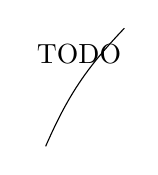
\begin{tikzpicture}
    \path (0,0)  edge [bend angle=10,bend right] node[label=TODO] {} (-1,-1.5);
\end{tikzpicture}

            \label{fig:assotiativitaet-von-wegen-a}
        }%
        \subfloat[$(\gamma_1 * \gamma_2) * \gamma_3$]{
            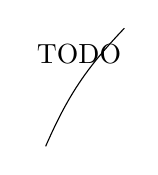
\begin{tikzpicture}
    \path (0,0)  edge [bend angle=10,bend right] node[label=TODO] {} (-1,-1.5);
\end{tikzpicture}

            \label{fig:assotiativitaet-von-wegen-b}
        }%
        \label{fig:assoziativitaet-von-wegen}
        \caption{Das Zusammensetzen von Wegen ist nicht assoziativ}
    \end{figure}

    Das Zusammensetzen von Wegen ist wegen Korollar~\ref{kor:homotope-wege}
    bis auf Homotopie assoziativ, da

    \[\gamma(t) = \begin{cases}
            \frac{1}{2} t   &\text{falls } 0 \leq t < \frac{1}{2}\\
            t - \frac{1}{4} &\text{falls } \frac{1}{2} \leq t < \frac{3}{4}\\
            2t - 1          &\text{falls } \frac{3}{4} \leq t \leq 1
        \end{cases}\]
\end{beweis}

\begin{korollar}\label{kor:bemerkung-10-6}
    Sei $X$ ein topologischer Raum, $a,b,c \in X$, $\gamma_1, \gamma_1'$
    Wege von $a$ nach $b$, $\gamma_2, \gamma_2'$ Wege von $b$ nach $c$.

    Sind $\gamma_1 \sim \gamma_1'$ und $\gamma_2 \sim \gamma_2'$, so
    ist $\gamma_1 * \gamma_2 \sim \gamma_1 ' * \gamma_2'$.
\end{korollar}

\begin{figure}
    \centering
    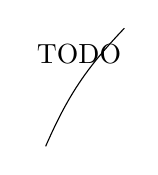
\begin{tikzpicture}
    \path (0,0)  edge [bend angle=10,bend right] node[label=TODO] {} (-1,-1.5);
\end{tikzpicture}

    \caption{Situation aus Korollar~\ref{kor:bemerkung-10-6}}.
    \label{fig:situation-bemerkung-10-6}
\end{figure}

\begin{beweis}
    Sei $H_i$ eine Homotopie zwischen $\gamma_i$ und $\gamma_i'$,
    $i=1,2$.

    Dann ist 
    \[H(t,s) := \begin{cases}
        H_1(2t, s)  &\text{falls } 0 \leq t \leq \frac{1}{2}\;\;\;\forall s \in I\\
        H_2(2t-1,s) &\text{falls } \frac{1}{2} \leq t \leq 1
    \end{cases}\]

    Homotopie zwischen $\gamma_1 * \gamma_2$ und $\gamma_1' * \gamma_2 '$ (!)
    \todo[inline]{Hier fehlt noch was}
\end{beweis}

\section{Fundamentalgruppe}
Für einen Weg $\gamma$ sei $[\gamma]$ seine \textbf{Homotopieklasse}\xindex{Homotopieklasse}.

\begin{definition}
    Sei $X$ ein topologischer Raum und $x \in X$. Sei außerdem
    \[\pi_1(X,x) := \Set{[\gamma] | \gamma \text{ ist Weg in } X \text{ mit } \gamma(0) = \gamma(1) = x}\]

    Durch $[\gamma_1] * [\gamma_2] : = [\gamma_1 * \gamma_2]$ wird
    $\pi_1(X,x)$ zu einer Gruppe. Diese Gruppe heißt \textbf{Fundamentalgruppe}\xindex{Fundamentalgruppe}
    in $X$ im Basispunkt $x$.
\end{definition}

\begin{bemerkung}
    Im $\mdr^2$ gibt es nur eine Homotopieklasse.
\end{bemerkung}

\begin{beweis}{Fundamentalgruppe ist eine Gruppe}
    \begin{enumerate}[label=\alph*)]
        \item Abgeschlossenheit folgt aus \todo{?}
        \item Assoziativität folgt aus Korollar~\ref{kor:assoziativitaet-von-zusammensetzen-von-wegen}
        \item Neutrales Element $e = [\gamma_0], \gamma_0(t) = x \;\;\; \forall t \in I$.

        $e * [\gamma] = [\gamma] = [\gamma] * e$, da $\gamma_0 * \gamma \sim \gamma$

        \begin{figure}
            \centering
            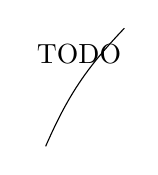
\begin{tikzpicture}
    \path (0,0)  edge [bend angle=10,bend right] node[label=TODO] {} (-1,-1.5);
\end{tikzpicture}

            \caption{Bis auf Parametrisierung sind $\gamma_0 * \gamma$ und $\gamma$ das selbe}.
            \label{fig:weg-zusammengesetzt-mit-neutralem-weg}
        \end{figure}
        \item Inverses Element  $[\gamma]^{-1} = [\overline{\gamma}] = [\gamma(1-t)]$, 
            denn $\overline{\gamma} * \gamma \sim \gamma_0 \sim \gamma * \overline{\gamma}$
    \end{enumerate}
\end{beweis}

\begin{beispiel}
    \begin{enumerate}[label=\arabic*)]
        \item $S^1 = \Set{z \in \mdc | |z| = 1} = \Set{(\cos \varphi, \sin \varphi) \in \mdr^2 | 0 \leq \varphi \leq 2 \pi}$

              $\pi_1 (S^1, 1) = \Set{[\gamma^k] | k \in \mdz} \cong \mdz$

              $[\gamma^k] \mapsto k$
        \item $\pi_1 (\mdr^2, 0) = \pi_1 (\mdr^2, x) = \Set{e}$ für jedes $x \in \mdr^2$
        \item $\pi_1 (\mdr^n, x) = \Set{e}$ für jedes $x \in \mdr^n$
        \item $G \subseteq \mdr^n$ \todo{hier fehlt was}heißt bzgl. $x \in G$, 
            wenn für jedes $y \in G$ auch die Strecke $[x, y] \subseteq G$
            ist.

            Für jedes sternförmige $G \subseteq \mdr^n$ ist
            $\pi_1(G,x) = \Set{e}$


            \begin{figure}[ht]
                \centering
                \subfloat[TODO]{
                    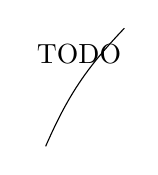
\begin{tikzpicture}
    \path (0,0)  edge [bend angle=10,bend right] node[label=TODO] {} (-1,-1.5);
\end{tikzpicture}

                    \label{fig:wege-zueinander-zusammenziehen}
                }\hspace{1em}%
                \subfloat[Sternförmiges Gebiet]{
                    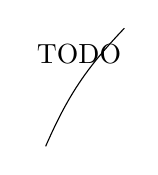
\begin{tikzpicture}
    \path (0,0)  edge [bend angle=10,bend right] node[label=TODO] {} (-1,-1.5);
\end{tikzpicture}

                    \label{fig:sternfoermiges-gebiet}
                }
                \label{fig:Gebiete}
                \caption{TODO}
            \end{figure}
        \item $\pi_1(S^2, x_0) = \Set{e}$, da im $\mdr^2$ alle Wege
              homotop zu $\Set{e}$ sind. Mithilfe der stereographischen
              Projektion kann von $S^2$ auf den $\mdr^2$ abgebildet
              werden.

              Dieses Argument funktioniert nicht mehr bei flächendeckenden
              Wegen!
    \end{enumerate}
\end{beispiel}

\begin{korollar}\label{kor:gruppenisomorphismus-wege}
    Sei $X$ ein topologischer Raum, $a,b \in X$, $\delta: I \rightarrow X$
    ein Weg von $a$ nach $b$.

    Dann ist die Abbildung
    \[\alpha: \pi_1 (X, a) \rightarrow \pi_1(X,b)\;\;\;[\gamma] \mapsto [\overline{\delta} * \gamma * \delta]\]
    ein Gruppenisomorphismus.
\end{korollar}

\begin{figure}
    \centering
    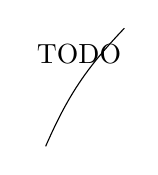
\begin{tikzpicture}
    \path (0,0)  edge [bend angle=10,bend right] node[label=TODO] {} (-1,-1.5);
\end{tikzpicture}

    \caption{Situation aus Korollar~\ref{kor:gruppenisomorphismus-wege}}.
    \label{fig:situation-gruppenisomorphismus-wege}
\end{figure}

\begin{beweis}
    \begin{align*}
        \alpha([\gamma_1] * [\gamma_2]) &= [\overline{\delta} * (\gamma_1 \gamma_2) * \delta]\\
        &= [\overline{\delta} * \gamma_1 * \delta * \overline{\delta} * \gamma_2 * \delta]
        &= [\overline{\delta} * \gamma_1 * \delta] * [\overline{\delta} * \gamma_2 * \delta]\\
        &= \alpha([\gamma_1]) * \alpha([\gamma_2])
    \end{align*}
\end{beweis}

% Die Übungsaufgaben sollen ganz am Ende des Kapitels sein.
\clearpage
\section*{Übungsaufgaben}
\addcontentsline{toc}{section}{Übungsaufgaben}

\begin{aufgabe}\label{ub5:aufg1}
    \todo{Todo}
\end{aufgabe}

